%% LaTeX2e class for student theses
%% thesis.tex
%% 
%% Karlsruhe Institute of Technology
%% Institute for Program Structures and Data Organization
%% Chair for Software Design and Quality (SDQ)
%%
%% Dr.-Ing. Erik Burger
%% burger@kit.edu
%%
%% See https://sdqweb.ipd.kit.edu/wiki/Dokumentvorlagen
%%
%% {$HeadURL$}
%% {$LastChangedDate$}
%% {$LastChangedRevision$}
%% {$LastChangedBy$}

%% Available page modes: oneside, twoside
%% Available languages: english, ngerman
%% Available modes: draft, final (see README)
\documentclass[twoside, english, draft]{sdqthesis}

%% --------------------------------
%% | Packages                     |
%% --------------------------------
\usepackage{todonotes}
\usepackage{amsmath}
\usepackage{amsfonts}
\usepackage{amssymb}


\usepackage{mathtools}

\usepackage{xcolor}
\definecolor{KITgreen}{rgb}{0,0.588,0.509}
\definecolor{KITgreen70}{rgb}{0.3,0.711,0.656}
\definecolor{KITgreen50}{rgb}{0.5,0.794,0.754}
\definecolor{KITgreen30}{rgb}{0.7,0.876,0.852}
\definecolor{KITgreen15}{rgb}{0.85,0.938,0.926}
\definecolor{KITblue}{rgb}{0.274,0.392,0.666}
\definecolor{KITblue70}{rgb}{0.492,0.574,0.766}
\definecolor{KITblue50}{rgb}{0.637,0.696,0.833}
\definecolor{KITblue30}{rgb}{0.782,0.817,0.9}
\definecolor{KITblue15}{rgb}{0.891,0.908,0.95}

\definecolor{KITblack}{rgb}{0,0,0}
\definecolor{KITblack70}{rgb}{0.3,0.3,0.3}
\definecolor{KITblack50}{rgb}{0.5,0.5,0.5}
\definecolor{KITblack30}{rgb}{0.7,0.7,0.7}
\definecolor{KITblack15}{rgb}{0.15,0.15,0.15}
\definecolor{KITpalegreen}{rgb}{0.509,0.745,0.235}
\definecolor{KITpalegreen70}{rgb}{0.656,0.821,0.464}
\definecolor{KITpalegreen50}{rgb}{0.754,0.872,0.617}
\definecolor{KITpalegreen30}{rgb}{0.852,0.923,0.77}
\definecolor{KITpalegreen15}{rgb}{0.926,0.961,0.885}
\definecolor{KITyellow}{rgb}{0.98,0.901,0.078}
\definecolor{KITyellow70}{rgb}{0.986,0.931,0.354}
\definecolor{KITyellow50}{rgb}{0.99,0.95,0.539}
\definecolor{KITyellow30}{rgb}{0.994,0.97,0.723}
\definecolor{KITyellow15}{rgb}{0.997,0.985,0.861}
\definecolor{KITorange}{rgb}{0.862,0.627,0.117}
\definecolor{KITorange70}{rgb}{0.903,0.739,0.382}
\definecolor{KITorange50}{rgb}{0.931,0.813,0.558}
\definecolor{KITorange30}{rgb}{0.958,0.888,0.735}
\definecolor{KITorange15}{rgb}{0.979,0.944,0.867}
\definecolor{KITbrown}{rgb}{0.627,0.509,0.196}
\definecolor{KITbrown70}{rgb}{0.739,0.656,0.437}
\definecolor{KITbrown50}{rgb}{0.813,0.754,0.598}
\definecolor{KITbrown30}{rgb}{0.888,0.852,0.758}
\definecolor{KITbrown15}{rgb}{0.944,0.926,0.879}
\definecolor{KITred}{rgb}{0.627,0.117,0.156}
\definecolor{KITred70}{rgb}{0.739,0.382,0.409}
\definecolor{KITred50}{rgb}{0.813,0.558,0.578}
\definecolor{KITred30}{rgb}{0.888,0.735,0.747}
\definecolor{KITred15}{rgb}{0.944,0.867,0.873}
\definecolor{KITlilac}{rgb}{0.627,0,0.47}
\definecolor{KITlilac70}{rgb}{0.739,0.3,0.629}
\definecolor{KITlilac50}{rgb}{0.813,0.5,0.735}
\definecolor{KITlilac30}{rgb}{0.888,0.7,0.841}
\definecolor{KITlilac15}{rgb}{0.944,0.85,0.92}
\definecolor{KITcyanblue}{rgb}{0.313,0.666,0.901}
\definecolor{KITcyanblue70}{rgb}{0.519,0.766,0.931}
\definecolor{KITcyanblue50}{rgb}{0.656,0.833,0.95}
\definecolor{KITcyanblue30}{rgb}{0.794,0.9,0.97}
\definecolor{KITcyanblue15}{rgb}{0.897,0.95,0.985}
\definecolor{KITseablue}{rgb}{0.196,0.313,0.549}
\definecolor{KITseablue70}{rgb}{0.437,0.519,0.684}
\definecolor{KITseablue50}{rgb}{0.598,0.656,0.774}
\definecolor{KITseablue30}{rgb}{0.758,0.794,0.864}
\definecolor{KITseablue15}{rgb}{0.879,0.897,0.932}

\usepackage{tikz}
\usepackage{pgfplots, pgfplotstable}
\usetikzlibrary{shapes.geometric, arrows, fit, positioning, backgrounds}


\usepackage[amsthm]{ntheorem}
\theoremstyle{break}
\theorembodyfont{\upshape}

\newtheorem{theorem}{Theorem}[section]
\newtheorem{definition}[theorem]{Definition}
\newtheorem{lemma}[theorem]{Lemma}
\newtheorem{example}[theorem]{Example}
\newtheorem{remark}[theorem]{Remark}

\usepackage{algorithm}
\usepackage{algorithmic}
\usepackage{stmaryrd}

\usepackage{hyphenat}

\usepackage{multirow}

\usepackage{caption}
\usepackage{subcaption}

\usepackage[nottoc]{tocbibind}
%\renewcommand{\chaptermark}[1]{\markboth{\thechapter.\ #1}{}}
\renewcommand{\tocetcmark}[1]{\thechapter.\ #1}
\renewcommand{\listoffigures}{
    \begingroup
    \tocchapter
    \tocfile{\listfigurename}{lof}
    \endgroup}
    
\interfootnotelinepenalty=10000

\usepackage[section]{placeins}

%% ---------------------------------
%% | Information about the thesis  |
%% ---------------------------------

%% Name of the author
\author{P. Samuel M. Teuber}

%% Title (and possibly subtitle) of the thesis
\title{Solving difficult SMT instances using\\
abstractions and incremental SMT solving}

%% Type of the thesis 
\thesistype{Bachelor's Thesis}

%% Change the institute here, ``IPD'' is default
\myinstitute{Institute of Theoretical Informatics (ITI)}

%% You can put a logo in the ``logos'' directory and include it here
%% instead of the SDQ logo
% \grouplogo{myfile}
%% Alternatively, you can disable the group logo
% \nogrouplogo

%% The reviewers are the professors that grade your thesis
\reviewerone{Prof. Dr. C. Sinz}
\reviewertwo{}

%% The advisors are PhDs or Postdocs
\advisorone{M.Sc. Marko Kleine Büning}
%% The second advisor can be omitted
\advisortwo{}

%% Please enter the start end end time of your thesis
\editingtime{15\textsuperscript{th} May 2019}{16\textsuperscript{th} September 2019}

\nogrouplogo

\settitle

%% --------------------------------
%% | Settings for word separation |
%% --------------------------------

%% Describe separation hints here.
%% For more details, see 
%% http://en.wikibooks.org/wiki/LaTeX/Text_Formatting#Hyphenation
\hyphenation{
% me-ta-mo-del
com-pu-ta-tio-nal
Ab-strak-tions-ver-fah-ren
}


%% --------------------------------
%% | Bibliography                 |
%% --------------------------------

%% Use biber instead of BibTeX, see README
\usepackage[citestyle=numeric,style=numeric,backend=biber,sorting=nyt]{biblatex}
\addbibresource{thesis.bib}

%% --------------------------------
%% | Hyperref                     |
%% --------------------------------
\hypersetup{final}

%% ====================================
%% ====================================
%% ||                                ||
%% || Beginning of the main document ||
%% ||                                ||
%% ====================================
%% ====================================
\begin{document}

%% --------------------------------
%% | Commands                     |
%% --------------------------------

\newcommand{\true}[0]{ \textbf{true} }
\newcommand{\false}[0]{ \textbf{false} }

\newcommand*\wc{{\mkern 2mu\cdot\mkern 2mu}}

%% Set PDF metadata
\setpdf

%% Set the title
\maketitle

%% The Preamble begins here
\frontmatter

%% LaTeX2e class for student theses: Declaration of independent work
%% sections/declaration.tex
%% 
%% Karlsruhe Institute of Technology
%% Institute for Program Structures and Data Organization
%% Chair for Software Design and Quality (SDQ)
%%
%% Dr.-Ing. Erik Burger
%% burger@kit.edu
%%
%% Version 1.3.3, 2018-04-17

\thispagestyle{empty}
\null\vfill
\noindent\hbox to \textwidth{\hrulefill} 
\todo{Place and Date!} 
I declare that I have developed and written the enclosed
thesis completely by myself, and have not used sources or means without
declaration in the text.\\
%% ---------------------------------------------
%% | Replace PLACE and DATE with actual values |
%% ---------------------------------------------
\textbf{PLACE, DATE}
\vspace{1.5cm}
%\dotfill
\hspace*{8.0cm}\\
\hspace*{2cm}(\theauthor) 
\cleardoublepage

\setcounter{page}{1}
\pagenumbering{roman}

%% ----------------
%% |   Abstract   |
%% ----------------
 
%% For theses written in English, an abstract both in English
%% and German is mandatory.
%%
%% For theses written in German, a German abstract is sufficient.
%%
%% The text is included from the following files:
%% - sections/abstract
\listoftodos


\includeabstract

%% ------------------------
%% |   Table of Contents  |
%% ------------------------
\tableofcontents

%% -----------------
%% |   Main part   |
%% -----------------

\mainmatter

%% LaTeX2e class for student theses
%% sections/content.tex
%% 
%% Karlsruhe Institute of Technology
%% Institute for Program Structures and Data Organization
%% Chair for Software Design and Quality (SDQ)
%%
%% Dr.-Ing. Erik Burger
%% burger@kit.edu
%%
%% Version 1.3.3, 2018-04-17

\chapter{Introduction}
\label{ch:introduction}
As an extension of the satisfiability problem for propositional logic formulae \cite{Marques-Silva-PropositionalSATSolving}, the satisfiability module theory (SMT) problem concerns with deciding numerous fragments of the first-order logic constraint by some \textit{Theory} $T$ \cite{Barrett-Tinelli-SMT}.
A SMT-Theory $T$ usually constraints the behaviour of certain uninterpreted functions or predicates of the first-order logic, but it may also syntactically constrain the language (e.g. by not allowing quantifiers).
Today, solving SMT problems has become a discipline of its own with many solving techniques relying in one way or another on a SAT solver in the background.
With SMT-LIB \cite{BarFT-SMTLIB} a unified interface to codify SMT instances has been developed that is supported by most if not all state-of-the-art SMT solvers.
\paragraph{}
Over the last decade a variety of approximation techniques have been introduced into the world of SMT solving and model checking with the objective of every approximation techniques being, to speed up the solving process thus reducing computational cost and avoiding exponential runtimes for common usecases.
Generally speaking, the techniques can be categorized into over-approximation (or abstraction) techniques like counterexample-guieded abstraction refinement (CEGAR) \cite{CEGAR} and lemmas on demand \cite{p6-brummayer} on the one hand, and under-approximation techniques like the ones used in UCLID \cite{Bryant2007_Chapter_DecidingBit-VectorArithmeticWi-UCLID}, but also in Boolector \cite{NiemetzPreinerBiere-JSAT15} on the other hand.
Usually, over-approximation techniques help in speeding up the solver's runtime for unsatisfiable SMT-instances, while under-approximation techniques help reducing the runtime of satisfiable instances \cite{Brummayer-PhD}. 
\paragraph{}
Although abstraction techniques have been successfully used for the array theory \cite{p6-brummayer} as well as the uninterpreted functions theory \cite{PreinerNiemetzBiere-DIFTS13,NiemetzPreinerBiere-FMCAD14}, there is little work on using over-approximations for the quantifier free bitvector logic (\texttt{QF\_BV} in SMT-LIB \cite{BarFT-SMTLIB}) outside the approach taken with UCLID \cite{Bryant2007_Chapter_DecidingBit-VectorArithmeticWi-UCLID}.
This thesis therefore takes up the topic of solving \enquote{difficult} bitvector SMT instances, like the ones provided in the \textit{LLBMC family of benchmarks} \cite{sc2017-proceedings}, using abstractions.
After an introduction to the topic and a short survey of current abstraction and solving approaches, we explain the pathway and intuition that led to the abstractions presented in chapter \ref{ch:refinement}.

\paragraph{Contributions}
Our contributions are twofold:
On the one hand we propose a theoretical framework allowing a simple proof of correctness for approximation techniques in SMT solving.
On the other hand we present an abstraction refinement technique for 3 functions of the \texttt{QF\_BV} SMT-Theory (namely \texttt{bvmul}, \texttt{bvsdiv} and \texttt{bvsrem}), proove their correctness and evaluate their performance using the relevant benchmark subset of 2018's SMT competition \cite{SMTCOMP18} and a prototype implementation of the abstraction refinement approach based on Boolector \cite{NiemetzPreinerBiere-JSAT15}.
\chapter{Related Work}
\label{ch:related_work}
While bit blasting (as described in the previous chapter) is the predominant approach for solving the \texttt{QF\_BV} theory and related theories, many approaches are being combined today in order to avoid bitblasting entire instances.
In this chapter a multitude of approaches used for solving the bitvector theory as well as solving related problems are being summarized. 

\section{Counterexample-Guieded abstractrion refinement (CEGAR)}
Counterexample-Guided abstraction refinement (CEGAR) was first proposed in the field of Software verification for the problem of verifying whether a given program $P$ adhears to some specification $\psi$ \cite{CEGAR}.\\
Given some program $P$ containing variables $V=\{v_1,\dots,v_n\}$ in domains $D_{v_1},\dots,D_{v_n}$ the set $D=D_{v_1}\times\dotsi\times D_{v_n}$ is the set of states of $P$. Let $p$ be some predicate then $\text{Atoms}\left(p\right)$ is the set of atomic formulae in $p$ and $\text{Atoms}\left(P\right)$ therefore is the set of atomic formulae in $P$. If some program state $d\in D$ satisfies some predicate $p$ we will write $d\vDash p$. A program defined this way can be directly transformed into a labeled Kripke-Structure $\mathcal{M}=\left(S,I,R,L\right)$ with $S=D$, $I\subseteq I$, $R \subseteq S \times S$, $L\colon S \to 2^{\text{Atoms}\left(P\right)}$ where $L\left(d\right) = \{ f \in \text{Atoms}\left(P\right) \mid d \vDash f \}$. The objective is then to compute whether $\mathcal{M}\vDash\psi$ id est whether the $P$'s Kripke-Structure $\mathcal{M}$ satisfies the specification $\psi$
\paragraph{Abstractions}
An abstraction in the CEGAR sense is a surjection $h\colon D \to \hat{D}$. An abstraction $h$ induces an equivalence relation on the set $D$ of program states with $d \equiv_h e$ iff $h\left(d\right) = h\left(e\right)$. Given a Kripke structure $\mathcal{M}$ and an abstraction $h$ the \textit{abstracted Kripke Structure} $\hat{\mathcal{M}} = \left(\hat{S},\hat{I},\hat{R},\hat{L}\right)$ is defined with:
\begin{itemize}
    \item $\hat{S} = \hat{D}$
    \item $\hat{d} \in \hat{I}$ iff $\exists d \in I\colon h\left(d\right) = \hat{d}$
    \item $\hat{R}\left(\hat{d_1},\hat{d_2}\right)$ iff $\exists d_1,d_2 \in D\colon h\left(d_1\right) = \hat{d_1} \land h\left(d_2\right) = \hat{d_2} \land R\left(d_1, d_2\right)$
    \item $\hat{L}\left(\hat{d}\right)=\bigcup\limits_{h\left(d\right)=\hat{d}} L\left(d\right)$
\end{itemize}

\begin{theorem}
    \label{theorem:related_work:cegar:sat}
    Let $h$ be an abstraction and $\psi$ some specification.
    Given that for every atomic formula $f$ in $\psi$ and for all $d,d' \in D$ the property $\left(d \equiv_h d'\right) \implies \left( d \vDash f \Leftrightarrow d' \vDash f \right)$ holds (we call this \enquote{$f$ respects $h$}), then:\\
    \begin{itemize}
        \item[(i)] $\hat{L}\left(\hat{d}\right)$ is consistent for all abstract states $\hat{d}$ in $\hat{M}$
        \item[(ii)] $\hat{\mathcal{M}}\vDash\psi \implies \mathcal{M} \vDash \psi$
    \end{itemize}
\end{theorem}
Do note that while correctness (as defined by $\psi$) of the abstract model $\hat{\mathcal{M}}$ implies correctness of the original model $\mathcal{M}$ a model might still be correct if $\hat{\mathcal{M}} \nvDash \psi$.

\paragraph{Initial abstraction}
Upon initialization of the solving process an initial abstraction $h$ is generated by grouping the variables $V=\{v_1,\dots,v_n\}$ into disjoint variable clusters $V = VC_1 \Dot{\cup} \dotsi \Dot{\cup} VC_n$. A variable cluster with variable $v_i$ contains any other variables $v_j$ which appear in the same atomic formulae as $v_i$ - clearly this induces an equivalence relation relation on the variables. For each variable cluster $VC_i=\{v_{i_1},\dots,v_{i_k}\}$ an abstraction is defined through:
\begin{flalign*}
   & h_i\left(d_1,\dots,d_k\right) = h_i\left(e_1,\dots,e_k\right)
    \text{ iff for all atomic formulae $f$}\\
    &\left(d_1,\dots,d_k\right) \vDash f \iff \left(e_1,\dots,e_k\right) \vDash f
\end{flalign*}

\paragraph{Handling counterexamples}
If the solver returns that $\hat{\mathcal{M}} \vDash \psi$ theorem \ref{theorem:related_work:cegar:sat} tells us that $\mathcal{M} \vDash \psi$. Otherwise the solver is assumend to return a counter example that can be checked on its correctness. More precisely it is necessary to check whether the counterexample is only possible in the abstracted structure $\hat{\mathcal{M}}$ or not. If the counterexample is caused by the abstraction and therefore \textit{spurious} a refinement step is made detailing the previous abstractions and the solver will run once again on this less-abstracted version of the problem \cite{CEGAR} until the counterexample is either correct or it is found that $\hat{\mathcal{M}}\vDash\psi$.
\paragraph{}
Ever since its introduction this approach of abstracting and refining has been used in wide range of applications including software verification \cite{CEGAR}, relational learning \cite{CEGAR-Relational-Learning} and SAT based planning \cite{CEGAR-Planning} as the core idea can be reused in most fields concerning with solving logic formulae.


%\section{STP}

\section{Boolector and Lemmas on Demand}
\label{par:related_work:boolector}
With Boolector \cite{Brummayer-Biere2009_Chapter_BoolectorAnEfficientSMTSolverF} another approach to over-approximation called \textit{Lemmas on Demand} was introduced to SMT solving. Boolector uses this extreme variant of lazy SMT solving for both solving array theory problems \cite{p6-brummayer} and uninterpreted function theory problems \cite{NiemetzPreinerBiere-FMCAD14}.
This is particularly interesting as Boolector interleaves over- and under-approximation techniques as can be seen in figure \ref{fig:related_work:boolector:scheme}.
Additionally Boolector makes heavy use of rewriting to solve easy bitvector theory instances - sometimes without using a SAT solver back-end at all.
\begin{figure}[h!]
    \centering
    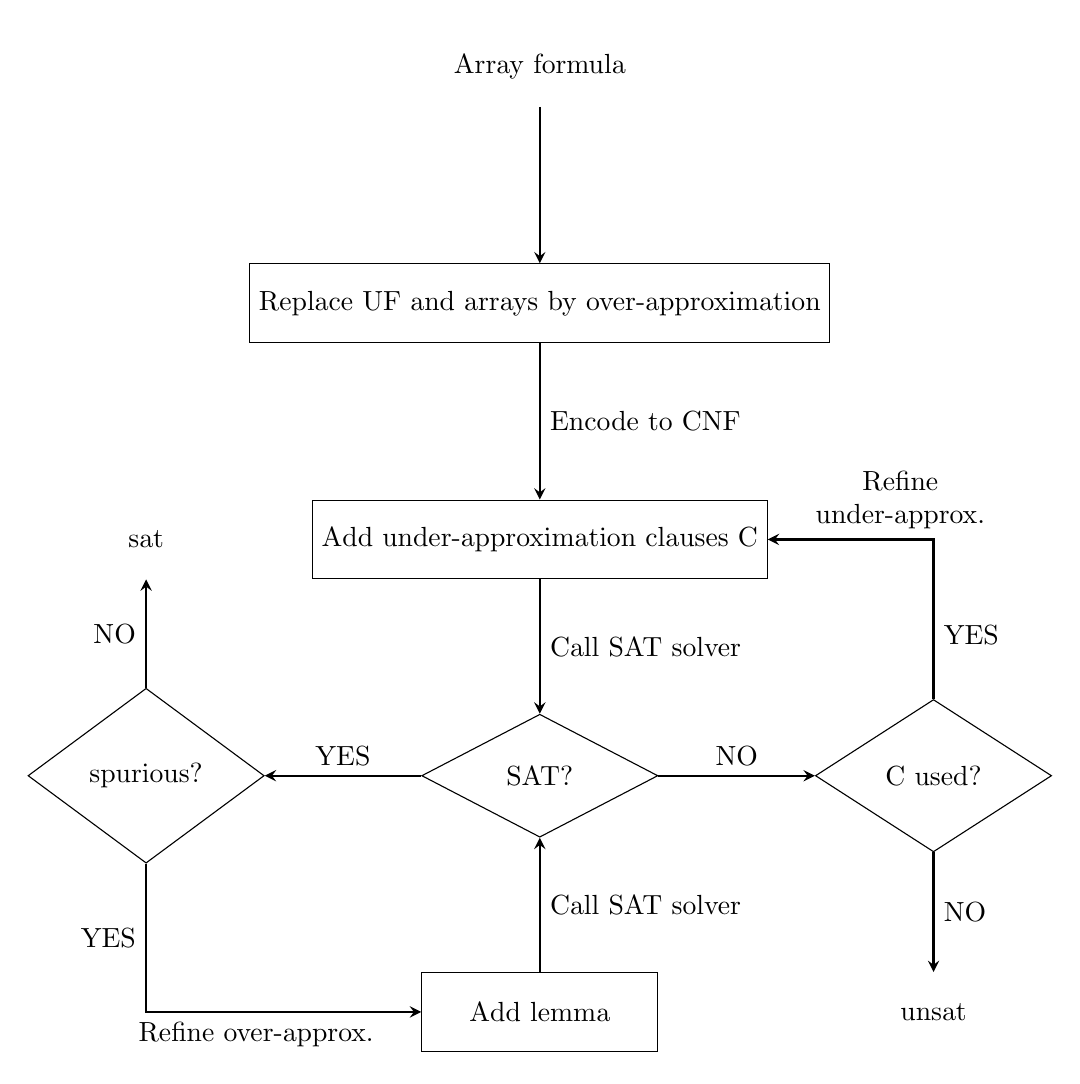
\begin{tikzpicture}[node distance=3cm]
    \tikzstyle{io} = [minimum width=3cm, minimum height=1cm, text centered]
    \tikzstyle{process} = [rectangle, minimum width=3cm, minimum height=1cm, text centered, draw=black]
    \tikzstyle{decision} = [diamond, minimum width=3cm, minimum height=1cm, text centered, draw=black]
    \tikzstyle{arrow} = [thick,->,>=stealth]
    
    \node (in) [io] {Array formula};
    \node (overapprox) [process, below of=in] {Replace UF and arrays by over-approximation};
    \node (underapprox) [process, below of=overapprox] {Add under-approximation clauses C};
    
    
    \node (issat) [decision, below of=underapprox] {SAT?};
    \node (isspurious) [decision, left of=issat,xshift=-2cm] {spurious?};
    \node (cused) [decision, right of=issat,xshift=2cm] {C used?};
    
    \node (satout) [io, above of=isspurious] {sat};
    \node (unsatout) [io, below of=cused] {unsat};
    
    \node (addlemma) [process, below of=issat] {Add lemma};
    
    \draw [arrow] (in) -- (overapprox);
    \draw [arrow] (overapprox) -- node[anchor=west] {Encode to CNF} (underapprox);
    \draw [arrow] (underapprox) -- node[anchor=west] {Call SAT solver} (issat);
    \draw [arrow] (issat) -- node[anchor=south] {YES} (isspurious);
    \draw [arrow] (issat) -- node [anchor=south] {NO} (cused);
    \draw [arrow] (isspurious) -- node[anchor=east] {NO} (satout);
    \draw [arrow] (isspurious) |- node[anchor=east,pos=0.25] {YES} node[anchor=north, pos=0.7] {Refine over-approx.} (addlemma);
    \draw [arrow] (addlemma) -- node[anchor=west] {Call SAT solver} (issat);
    
    \draw [arrow] (cused) -- node[anchor=west] {NO} (unsatout);
    
    \draw [arrow] (cused) |- node[anchor=west,pos=0.2] {YES} node[anchor=south,pos=0.6,align=center] {Refine\\under-approx.} (underapprox);
    
    \end{tikzpicture}
    \caption{Interleaving over- and under-approximation techniques in Boolector as presented in \cite{Brummayer-PhD}}
    \label{fig:related_work:boolector:scheme}
\end{figure}

\paragraph{Rewriting}
SMT formulae passed to Boolector are rewritten in 3 levels \cite{Brummayer-Biere2009_Chapter_BoolectorAnEfficientSMTSolverF}. In a first step very basic logic rules are applied during formula construction. In a second step global term substitution is performed on a topologically sorted DAG representation of the formula set. In a third and last step arithmetic normalization is performed.

\paragraph{Under-Approximation}
Boolector makes use of under-approximation on the CNF level by adding assumptions to the SAT solver instance\cite{Brummayer-PhD}. Boolector restricts the \textit{effective bitwidth} of a given bitvector to a smaller size which is then sign extended (or sometimes zero extended) to reach the original bitsize. Using a newly introduced assumption variable $e$ this behaviour can be (de)activated as needed each run through the SAT solvers assumption interface by adding/removing an activation clause $e$ or $\neg e$. On the one hand the additional constraints reduce the search-space size and thereby help to potentially speed up the solver's search. On the other hand the additional constraints lead the solver towards smaller, usually better understandable models.

\paragraph{Lemmas on Demand}
Boolector makes use of over-approximation for solving the array \cite{p6-brummayer} and uninterpreted function (UF) theories \cite{PreinerNiemetzBiere-DIFTS13}. We will now explain the idea behind this extreme variant of lazy SMT solving based on the uninterpreted function case. For it's extension to arrays the reader is referred to \cite{p6-brummayer}. While not relevant for this work \cite{PreinerNiemetzBiere-DIFTS13} also explains how lemmas on demand can be used for lambda expressions. 
\par
For its initial abstraction every UF applications is replaced by a fresh bitvector variable. Afterwards the problem can be eagerly encoded as a SAT problem. If the SAT solver returns unsatisfiability the original problem is unsatisfiable, too. If on the other hand, the SAT solver returns a satisfying interpretation $\mathcal{I}$ we must now check whether the corresponding SMT interpretation $t\left(\mathcal{I}\right)$ interpretation is consistent with the uninterpreted function's theory. More precisely we must check, whether for every function $f$ its applications $f\left(\overline{x_1}\right),\dots,f\left(\overline{x_{m_{f}}}\right)$ are consistent with the (\ref{eq:preliminaries:smt:euf}) axiom.
\par
If it is found that for two UF applications $t=f\left(a_1,\dots,a_n\right)$ and $s=f\left(b_1,\dots,b_n\right)$
the axiom is not respected (i.e. $a_i=b_i$ for all $i\in\llbracket1,n\rrbracket$ but $s\neq t$) an additional lemma encoding this constraint will be added. For this the shortest paths $p^s$ and $p^t$ from the function application $s$ (and $t$) to $f$ are calculated and all \textit{ite} conditions $c_0^s,\dots,c_j^s$ ($c_0^t,\dots,c_k^t$) on the paths evaluating to $\blacksquare$ under $t\left(\mathcal{I}\right)$ as well as all \textit{ite} conditions $d_0^s,\dots,d_l^s$ ($d_0^t,\dots,d_m^t$) on the paths evaluating to $\square$ under $t\left(\mathcal{I}\right)$ are collected. Using this information the following lemma is added to the SAT instance:
\[
\left(\bigwedge\limits_{i=0}^{j}c_i^s \land \bigwedge\limits_{i=0}^{k}c_i^t \land \bigwedge\limits_{i=0}^{l} \neg c_i^s \land \bigwedge\limits_{i=0}^{m} \neg c_i^t \land \bigwedge\limits_{i=0}^{n} a_i=b_i \right) \implies s=t
\]
As can be seen in the success of Boolector this approach proved very effective in solving both the Array Theory as well as the UF theory. The technique can be further optimized by only refining those UF applications which are actually relevant for the current satisfying counterexample \cite{NiemetzPreinerBiere-FMCAD14}.

\paragraph{Overflow Detection}
Boolector implements efficiently encoded predicates for overflow detection in addition, substraction, multiplication and division \cite{Brummayer-PhD}. Let $L\left(a\right)$ be the number of leading bits (zero or one) for some bitvector $a$. For a signed multiplication $r=a*b$ an overflow occurs iff $L\left(a\right) + L\left(b\right) < n$ or $r\left[n\right] \oplus r\left[n-1\right]$ \cite{schulteGokMulOv}. This result allows to check a signed multiplication for overflow issues by only calculating the first $n+1$ multiplication bits in contrast to $2n$ bits for the naive encoding. Similar predicates are available for all basic arithmetic operations.7

\section{UCLID}
Though using another technique, \textsc{UCLID} \cite{Bryant2007_Chapter_DecidingBit-VectorArithmeticWi.pdf} was one of the SMT solvers which pioneered the interleaving of Over- and Under-Approximations using abstractions. Given an input formula $\phi$ the \textsc{UCLID} solver constructs an SMT under-approximation $\underline{\phi}$. The formula is usually generated by restricting variables to their sign-extended versions of a smaller bit size as previously seen in Boolector (i.e. $v_nv_{n-1}\dotsi v_1$ becomes $v_mv_m\dotsi v_m v_{m-1}\dotsi v_1$.) This formula $\underline{\phi}$ is then eagerly encoded and passed to a SAT solver. The SAT solver can produce one of two outcomes:

\paragraph{SAT} In case the SAT solver finds a model such that $t\left(\mathcal{I}\right)\vDash\underline{\phi}$ the solver returns sat as $t\left(\mathcal{I}\right)\vDash\phi$. In this case \textsc{UCLID} can potentially speed up the SAT solver's runtime due to the reduced search space in the under-approximation $\underline{\phi}$

\paragraph{UNSAT} In case the SAT solver returns an unsatisfiability result \textsc{UCLID} uses the UNSAT-Core returned by the solver to extract the the SAT-formulae which produced the contradiction. Only based on these formulae (thereby leaving out all formulae of the instance that are not part of the UNSAT result) an over-approximation $\overline{\phi}$ is built. In contrast to $\underline{\phi}$ this over-approximation does in no way restrict the bitwidth of the input variables. The SAT solver is then passed $\overline{\phi}$. If the SAT solver still returns unsatisfiability \textsc{UCLID} returns unsat. In case the solver returns satisfiability the under-approximation $\underline{\phi}$ is refined (usually increasing the bitwidth) and a second iteration is started.
\par
For unsatisfiable instances \textsc{UCLID} takes advantage of cases where a small number of formulae can produce the contradiction and makes the SAT-solver only look at these formulae thereby potentially improving the solver's performance.

\paragraph{Notes}
UCLID
Interleaving under- and overapproximations
Works for extracting unsat cores of under approximations that might be able to produce a contradiction in main problem
-> We will soon see that this methodology does not work for some of the concerned problems (specifically this methodology wouldn't yield good results for modmul given its the core size)

\chapter{Benchmark Analysis}
\label{ch:benchmark_analysis}
- modmul-32 produces a \cite{sc2017-proceedings}


\chapter{Refinement approach}
\label{ch:refinement}
In this chapter we present an abstraction procedure for the quantifier free bitvector theory (\texttt{QF\_BV}).
The approach substitutes applications of specific functions (here \texttt{bvmul}, \texttt{bvsdiv} and \texttt{bvsrem}) by \textit{abstractions} defined on the \texttt{QF\_UFBV} theory.
During the solving process, an instance's abstractions are iteratively refined until the SAT solver either returns unsatisfiability or satisfiability with correct assignments.

\section{Abstraction scheme}
In the SMT-LIB standard \cite{BarFT-SMTLIB} for \texttt{QF\_BV} the functions examined in this work (i.e., \texttt{bvmul}, \texttt{bvsdiv} and \texttt{bvsrem}) support \textit{overloading} in the sense that a single function symbol like \texttt{bvmul} supports multiple ranks. Multiplication for example is supported for any bitwidth.
To simplify the explanations in the following sections one can think of $\texttt{bvmul}^r$ as the \texttt{bvmul} operation of rank $r$ thereby avoiding the issue of overloading.

\begin{definition}[Approximation]
Given some theory $T=\left(\Sigma,A\right)$ and some function symbol $\texttt{op}\in\Sigma^F$ with $\mathcal{s}^F\left(\texttt{op}\right)=\sigma_1\dotsi\sigma_n\sigma$ and $n\geq1$, a $T$-approximation for \texttt{op} consists of:
\begin{itemize}
    \item a new uninterpreted function symbol $ap_{\texttt{op}}$ with $\mathcal{s}^F\left(\texttt{op}\right) = \mathcal{s}^F\left(ap_{\texttt{op}}\right)$; and
    \item a mapping $\mathcal{A}_{\texttt{op}}\colon \textsc{Term}^\Sigma_{\sigma_1}\times\dotsi\times\textsc{Term}^\Sigma_{\sigma_n} \to 2^{\textsc{For}^1_T}$.
\end{itemize}
A $T$-approximation can therefore be written as a tuple $\left(ap_{\texttt{op}}, \mathcal{A}_{\texttt{op}}\right)$
\end{definition}
We can now define properties that a $T$-approximation might have. This will be useful to prove the correctness of our abstraction procedure later on

\begin{definition}[Sound $T$-approximation]
    \label{def:refinement_approach:abstraction_scheme:soundness}
Given some theory $T=\left(\Sigma,A\right)$ a $T$-approximation $\left(ap_{\texttt{op}}, \mathcal{A}_{\texttt{op}}\right)$ is sound iff for all
$\overline{x}\in Dom
\footnote{$Dom$ is the domain of a given function. In this case $Dom\left(\mathcal{A}_{\texttt{op}}\right) = \textsc{Term}^\Sigma_{\sigma_1}\times\dotsi\times\textsc{Term}^\Sigma_{\sigma_n}$}
\left(\mathcal{A}_{\texttt{op}}\right)$ the following property holds:\\
For all $T$-interpretation $\mathcal{I}$ with $\mathcal{I}\vDash\mathcal{A}_{\texttt{op}}\left(\overline{x}\right)$ there is also
$\mathcal{I}\vDash ap_{\texttt{op}}\left(\overline{x}\right) \doteq \texttt{op}\left(\overline{x}\right)$.
\end{definition}

\begin{definition}[Complete $T$-approximation]
\label{def:refinement_approach:abstraction_scheme:completeness}
Given some theory $T=\left(\Sigma,A\right)$ a $T$-approximation $\left(ap_{\texttt{op}}, \mathcal{A}_{\texttt{op}}\right)$ is complete iff for all $\overline{x}\in Dom\left(\mathcal{A}_{\texttt{op}}\right)$ the following property holds:\\
For all $T$-interpretations $\mathcal{I}$ with $\mathcal{I}\vDash ap_{\texttt{op}}\left(\overline{x}\right) \doteq \texttt{op}\left(\overline{x}\right)$ there is also
$\mathcal{I}\vDash\mathcal{A}_{\texttt{op}}\left(\overline{x}\right)$.
\end{definition}

\begin{example}
For readability let $\texttt{f} \coloneqq \texttt{mul}^{\mathbf{BV}_2\mathbf{BV}_2\mathbf{BV}_2}$ be the 2-bit multiplication function as defined in \texttt{QF\_BV}.\\
Example for a sound approximation:
\[
    \mathcal{A}_\texttt{f}\left(x_1,x_2\right) 
    \coloneqq \{
    ab_\texttt{f}\left(x_1,x_2\right) \doteq 0, \left(x_1\doteq 0 \lor x_2 \doteq 0\right)
    \}
\]
Example for a complete approximation:
\[
    \mathcal{A}_\texttt{f}\left(x_1,x_2\right) 
    \coloneqq \{
    \left(x_1\doteq 0 \lor x_2 \doteq 0\right) \implies ab_\texttt{f}\left(x_1,x_2\right) \doteq 0
    \}
\]
Example for a sound and complete approximation:
\[
\mathcal{A}_\texttt{f}\left(x_1,x_2\right) 
        \coloneqq \{
        ab_\texttt{f}\left(x_1,x_2\right) \doteq \texttt{f}\left(x_1,x_2\right)
        \}
\]
\end{example}
Essentially a sound $T$-approximation describes an under-approximation and a complete $T$-approximation describes an over-approximation of some function \texttt{op}. Using the notions defined above we can now define an abstraction scheme which iteratively refines an over-approximation until the abstraction converges into an exact description of the given function.
\begin{definition}[Abstraction Scheme]
Given some theory $T=\left(\Sigma,A\right)$ and some function symbol $\texttt{op}\in\Sigma^F$ of arity greater $0$, a $T$-abstraction scheme is a finite, totally ordered set of $\ T$-approximations \[
\mathcal{AS}_{\texttt{op}} = \{ \left(ab_{\texttt{op}}, \mathcal{A}^1_{\texttt{op}}\right),\dots,\left(ab_{\texttt{op}}, \mathcal{A}^k_{\texttt{op}}\right) \}
\]
where:
\begin{itemize}
    \item For every $i\in\llbracket1,k\rrbracket$: $\mathcal{A}^i_{\texttt{op}}$ is a complete $T$-approximation of \texttt{op}
    \item $\mathcal{C}_{\texttt{op}}\left(\overline{x}\right)\coloneqq\left(\bigcup\limits_{\left(\wc,\mathcal{A}\right)\in\mathcal{AS}_{\texttt{op}}} \mathcal{A}\left(\overline{x}\right)\right)$ is a sound $T$-approximation of \texttt{op}
    \footnote{
        Just like all previous $T$-approximations $\mathcal{C}_{\texttt{op}}$ is defined as
        $\mathcal{C}_{\texttt{op}}\colon \textsc{Term}^\Sigma_{\sigma_1}\times\dotsi\times\textsc{Term}^\Sigma_{\sigma_n} \to 2^{\textsc{For}^1_T}$ for a function symbol \texttt{op} of rank $\sigma_1\dotsi\sigma_n\sigma$
    }
\end{itemize}
\end{definition}

\begin{lemma}[Completeness of Abstraction Schemes]
    \label{lemma:refinement_approach:abstraction_scheme:as_completeness}
Given some $T$-approximation scheme 
$\mathcal{AS}_{\texttt{op}} = \{ \left(ab_{\texttt{op}}, \mathcal{A}^1_{\texttt{op}}\right),\dots,\left(ab_{\texttt{op}}, \mathcal{A}^k_{\texttt{op}}\right) \}$
with the properties defined above we can show that:\\
$\mathcal{C}_{\texttt{op}}$ is a complete $T$-approximation of \texttt{op}.
\begin{proof}
Let $\overline{x}$ be an arbitrary input vector for \texttt{op}.\\
By definition we know that for any $T$-interpretation $\mathcal{I}$ with $\mathcal{I} \vDash ap_{\texttt{op}}\left(\overline{x}\right) \doteq \texttt{op}\left(\overline{x}\right)$ there is also $\mathcal{I} \vDash \mathcal{A}^i_{\texttt{op}}\left(\overline{x}\right)$ for all $i\in\llbracket1,k\rrbracket$ as all approximations $\mathcal{A}^i_{\texttt{op}}$ are complete.\\
Therefore,
\[
    \mathcal{I} \vDash \bigcup\limits_{\left(\wc,\mathcal{A}\right)\in\mathcal{AS}_{\texttt{op}}} \mathcal{A}\left(\overline{x}\right)
    \text{ (i.e., }\mathcal{I} \vDash \mathcal{C}_{\texttt{op}}\left(\overline{x}\right)\text{)}
\]
which implies that $\mathcal{C}_{\texttt{op}}$ is a complete $T$-approximation, too.
\end{proof}
\end{lemma}

\begin{lemma}[Soundness/Completeness through Implication]
    \label{lemma:refinement_approach:abstraction_scheme:implication}
    Given some theory $T=\left(\Sigma,A\right)$ and a $T$-approximation $\left(ap_{\texttt{op}}, \mathcal{A}_{\texttt{op}}\right)$:\\
    If for all interpretations $\mathcal{I}$ and all $\overline{x}\in Dom\left(\mathcal{A}_{\texttt{op}}\right)$
    \[
        \mathcal{A}_{\texttt{op}}\left(\overline{x}\right) \implies ap_{\texttt{op}}\left(\overline{x}\right) \doteq \texttt{op}\left(\overline{x}\right)
    \]
    then $\left(ap_{\texttt{op}}, \mathcal{A}_{\texttt{op}}\right)$ is sound.\\
    If for all interpretations $\mathcal{I}$ and all $\overline{x}\in Dom\left(\mathcal{A}_{\texttt{op}}\right)$
    \[
        ap_{\texttt{op}}\left(\overline{x}\right) \doteq \texttt{op}\left(\overline{x}\right) \implies \mathcal{A}_{\texttt{op}}\left(\overline{x}\right)
    \]
    then $\left(ap_{\texttt{op}}, \mathcal{A}_{\texttt{op}}\right)$ is complete.
    \begin{proof}
        The proof follows directly from definitions \ref{def:refinement_approach:abstraction_scheme:soundness} (\ref{def:refinement_approach:abstraction_scheme:completeness}).\\
        Given for some formula the soundness (completeness) formula above holds for all $\mathcal{I}$ and $\overline{x}$:\\
        For any interpretation $\mathcal{I}$ where
            $\mathcal{I}\nvDash\mathcal{A}_{\texttt{op}}\left(\overline{x}\right)$
            ($\mathcal{I}\nvDash ap_{\texttt{op}}\left(\overline{x}\right) \doteq \texttt{op}\left(\overline{x}\right)$)
            the definition for soundness (completeness) is already fulfilled.\\
        In case for some interpretation $\mathcal{I}$ it holds that 
            $\mathcal{I}\vDash\mathcal{A}_{\texttt{op}}\left(\overline{x}\right)$
            ($\mathcal{I}\vDash ap_{\texttt{op}}\left(\overline{x}\right) \doteq \texttt{op}\left(\overline{x}\right)$)
        then we know through the formula above that
            $\mathcal{I}\vDash ap_{\texttt{op}}\left(\overline{x}\right) \doteq \texttt{op}\left(\overline{x}\right)$
            ($\mathcal{I}\vDash\mathcal{A}_{\texttt{op}}\left(\overline{x}\right)$)
        which implies that the approximation is, by definition, sound (complete).


    \end{proof}
\end{lemma}

\begin{theorem}[Correctness of abstraction approach]
\label{theorem:abstractions:scheme:equivalence}
Let $T=\left(\Sigma,A\right)$ be some theory with $\texttt{op}\in\Sigma^F$, $\mathcal{s}^F\left(\texttt{op}\right)=\sigma_1\dotsi\sigma_n\sigma$ and $n\geq1$.\\
Let further $\Phi$ be an arbitrary $\Sigma$-formula containing some function application $\texttt{op}\left(\overline{x}\right)$.\\
Given some term $t\in\textsc{Term}_\sigma^\Sigma$ we define $\Phi\left[\texttt{op}\left(\overline{x}\right)\mapsto t \right]$ as the formula where $\texttt{op}\left(\overline{x}\right)$ was replaced by $t$ in $\phi$.\\
For any $T$-abstraction scheme $\mathcal{AS}_{\texttt{op}}$ with function symbol $ab_{\texttt{op}}$ the following property holds:\\
There exists a $T$-interpretation $\mathcal{I}_{\Phi}$ that is a $T$-model for $\Phi$ iff there exists a $T$-interpretation $\mathcal{I}_{\mathcal{A}}$ that is a $T$-model for 
\[
\Psi \coloneqq \Phi\left[ \texttt{op}\left(\overline{x}\right) \mapsto ab_{\texttt{op}}\left(\overline{x}\right) \right] \land \bigwedge\limits_{\left(\wc,\mathcal{A}\right)\in\mathcal{AS}_{\texttt{op}}} \mathcal{A}\left(\overline{x}\right)
\]
\begin{proof}
The theorem will be proved in 2 directions. For each direction we will construct a suitable interpretation given the premise interpretation.
\begin{itemize}
    \item[$\Rightarrow$] Let $\mathcal{I}_{\Phi}$ be a $T$-model for $\Phi$.\\
        We will now build a model $\mathcal{I}_{\mathcal{A}}$ by extending $\mathcal{I}_{\Phi}$ so that $\mathcal{I}_\mathcal{A}\left(ab_{\texttt{op}}\left(\overline{x}\right)\right)$
        evaluates to $\mathcal{I}_{\Phi}\left(\texttt{op}\left(\overline{x}\right)\right)$.\\
        We then know that $\mathcal{I}_{\mathcal{A}} \vDash ap_{\texttt{op}}\left(\overline{x}\right) \doteq \texttt{op}\left(\overline{x}\right)$
        and the completeness proofed in Lemma \ref{lemma:refinement_approach:abstraction_scheme:as_completeness} tells us that thereby
        $\mathcal{I}_{\mathcal{A}} \vDash \mathcal{A}_{\texttt{op}}\left(\overline{x}\right)$.
        Therefore 
        \[
            \mathcal{I}_{\mathcal{A}} \vDash\Phi\left[ \texttt{op}\left(\overline{x}\right) \mapsto ab_{\texttt{op}}\left(\overline{x}\right) \right] \land \bigwedge\limits_{\left(\wc,\mathcal{A}\right)\in\mathcal{AS}_{\texttt{op}}} \mathcal{A}\left(\overline{x}\right)
        \]
    \item[$\Leftarrow$]  Let $\mathcal{I}_{\mathcal{A}}$ be a $T$-model for $\Psi$.\\
        The abstraction scheme definition tells us that
        \[
            \mathcal{I}_{\mathcal{A}} \vDash \bigwedge\limits_{\left(\wc,\mathcal{A}\right)\in\mathcal{AS}_{\texttt{op}}} \mathcal{A}\left(\overline{x}\right)
        \] 
        also yields $\mathcal{I}_{\mathcal{A}} \vDash ap_{\texttt{op}}\left(\overline{x}\right) \doteq \texttt{op}\left(\overline{x}\right)$ through the soundness property.\\
        This implies that $\mathcal{I}_{\mathcal{A}} \vDash \Phi$.
\end{itemize}
\end{proof}
\end{theorem}

\paragraph{Abstraction approach}
In the following sections abstraction schemes for three function symbols of the \texttt{QF\_BV} theory will be presented.
In order to proof that the abstractions are actually valid we will:
\begin{itemize}
    \item[(A)] Proof the completeness of any approximation proposed
    \item[(B)] Proof the soundness of each abstraction scheme
\end{itemize}
The abstractions can then be used to build a decision procedure like the one described in Algorithm \ref{algorithm:refinement_approach:abstraction_scheme:refinement}
As can be seen in Theorem \ref{theorem:abstractions:scheme:equivalence}, (A) and (B) will be enough to prove that the abstraction schemes yield correct results when used in such a decision procedure.\\


\begin{algorithm}
    \caption{Decision procedure for QF\_BV abstractions}
    \begin{algorithmic}
    \label{algorithm:refinement_approach:abstraction_scheme:refinement}
    \REQUIRE $\phi \in \textsc{For}^1_{QF\_BV}$
    \STATE abstractions$ \leftarrow \langle\rangle$
    \STATE operations$ \leftarrow \langle\rangle$
    \FORALL{$\texttt{op}\in\Sigma^F$}
        \IF{\texttt{op} needs refinement}
            \FORALL{$\texttt{op}\left(\overline{x}\right)$ in $\phi$}
                \STATE $\phi \leftarrow \phi\left[\texttt{op}\left(\overline{x}\right) \mapsto ab_\texttt{op}\left(\overline{x}\right)\right]$
                \STATE abstractions.push$\left(\mathcal{AS}_\texttt{op}\right)$
                \STATE operations.push$\left( \texttt{op}\left(\overline{x}\right) \right)$
            \ENDFOR
        \ENDIF
    \ENDFOR
    \STATE \texttt{ADD\_CLAUSES($\phi$)}
    \LOOP
    \STATE $r \leftarrow $\texttt{SAT($\phi$)}
    \IF{\NOT $r$}
        \PRINT unsat
    \ELSE
        \STATE correct $\leftarrow \TRUE$
        \FORALL{$\texttt{op}\left(\overline{x}\right)$ in operations}
            \IF{\NOT $\texttt{op}\left(\overline{x}\right)$ assignment is correct}
                \STATE correct $\leftarrow \FALSE$
            \ENDIF
        \ENDFOR
        \IF{correct}
            \PRINT sat
        \ELSE
            \FORALL{$\mathcal{AS}$ in abstractions}
                \STATE \texttt{ADD\_CLAUSES($\mathcal{AS}$.pop())}
                \COMMENT{Add next approximation to for $\mathcal{AS}$ to instance}
            \ENDFOR
        \ENDIF
    \ENDIF
    \ENDLOOP
    \end{algorithmic}
\end{algorithm}

\section{Abstracting \texttt{bvmul}}
The abstraction scheme for \texttt{bvmul} is devided into four stages:
The first stage describes the behaviour of \texttt{bvmul} for various common cases (like factors 0 and 1);
the second stage defines intervals for the result value given the intervals of the multiplication factors;
the third stage introduces relations between \texttt{bvmul} and other functions (specifically \texttt{bvsdiv} and \texttt{bvsrem});
the fourth stage finally adds full multiplication for certain intervals of the factors.

\paragraph{Overflow detection}
The \texttt{bvmul} function essentially behaves just like \enquote{regular} integer multiplication for any input value
which doesn't produce an overflow.
Upon overflow however, \texttt{bvmul} oftentimes behaves strangely as behaviour in modern C compilers is usually undefined
and behaviour in SMT-LIB - though well defined - is difficult to model mathematically the same way it is done for \enquote{regular} multiplication.
For many of the abstractions proposed in this chapter it is therefore essential to detect overflows.
As we have already seen in section \ref{par:related_work:boolector}, Boolector supports a predicate to detect signed and unsigned multiplication overflows.
The issue with this predicate is however that we have to calculate the first $w+1$ steps of multiplication given bitvectors of width $w$.
This is rather impractical when one only event wants to abstract the first $w$ steps of multiplication.
Therefore a predicate with no need for a multiplication unit was needed.
Obviously such a predicate without a multiplication unit, while complete, might not be sound - i.e., while every overflow might be detected,
this predicate might detect more overflows than actually exist.
The methodology used here is based on \cite{Warren-HackersDelight} where another methodology for detecting overflows by counting the leading bits (ones or zeros)
is proposed:
The predicate ensures that there are at least $w+2$ leading bits for any multiplication of 2 negative numbers and at least $w+1$ leading bits for any other multiplication.
While excluding a few cases with no overflows this predicate is never true for a pair of factors which results in an overflow.
The corresponding predicate is defined in Definition \ref{def:refinement_approach:bvmul:noov} and will be used on multiple occasions in the following sections.
\begin{definition}[$noov$ predicate]
    We define a Boolean function $noov: \{0,1\}^w \times \{0,1\}^w \rightarrow \{0,1\}$ with
    \label{def:refinement_approach:bvmul:noov}
    \begin{align*}
        noov\left(a, b\right)
        = &\bigvee\limits_{n=0}^{w-1}
            \left(
            \bigwedge\limits_{i=0}^{n} \neg a[w-i-1]
            \land
            \bigwedge\limits_{i=n}^{w-1} \neg b[i]
            \right) \lor\\
            &\bigvee\limits_{n=0}^{w-1}
            \left(
            \bigwedge\limits_{i=0}^{n} a[w-i-1]
            \land
            \bigwedge\limits_{i=n}^{w-1} \neg b[i]
            \right) \lor\\
            &\bigvee\limits_{n=0}^{w-1}
            \left(
            \bigwedge\limits_{i=0}^{n} \neg a[w-i-1]
            \land
            \bigwedge\limits_{i=n}^{w-1} b[i]
            \right) \lor\\
            &\bigvee\limits_{n=0}^{w-2}
            \left(
            \bigwedge\limits_{i=0}^{n} a[w-i-2]
            \land
            \bigwedge\limits_{i=n}^{w-2} b[i]
            \land a[w-1]
            \land b[w-1]
            \right)
    \end{align*}
\end{definition}

\subsection{Simple cases}
\label{subsec:refinement_approach:bvmul:simple}
For a multiplication instance $ab_\texttt{bvmul}\left(x,y\right)$ of factors $x$ and $y$ with bitwidth $w$ we define the following constraints:
\begin{flalign}
    \left(x \doteq 0\right) &\Rightarrow && \left(ab_\texttt{bvmul}\left(x,y\right) \doteq 0\right)
        &\label{align:refinement_approach:bvmul:simple:zero1}\\
    \left(y \doteq 0\right) &\Rightarrow && \left(ab_\texttt{bvmul}\left(x,y\right) \doteq 0\right)
        &\label{align:refinement_approach:bvmul:simple:zero2}\\
    \left(x \doteq 1\right) &\Rightarrow && \left(ab_\texttt{bvmul}\left(x,y\right) \doteq y\right)
        &\label{align:refinement_approach:bvmul:simple:one1}\\
    \left(y \doteq 1\right) &\Rightarrow && \left(ab_\texttt{bvmul}\left(x,y\right) \doteq x\right)
        &\label{align:refinement_approach:bvmul:simple:one2}\\
    \left(x \doteq -1\right) &\Rightarrow && \left(ab_\texttt{bvmul}\left(x,y\right) \doteq -y\right)
        &\label{align:refinement_approach:bvmul:simple:neg1}\\
    \left(y \doteq -1\right) &\Rightarrow && \left(ab_\texttt{bvmul}\left(x,y\right) \doteq -x\right)
        &\label{align:refinement_approach:bvmul:simple:neg2}\\
    noov(x,y) &\Rightarrow && 
        \left( \neg x[w-1] \land \neg y[w-1] \right)
            \Rightarrow
            \left(ab_\texttt{bvmul}\left(x,y\right) \geq 0\right)
                &\label{align:refinement_approach:bvmul:simple:bothPos}\\
            && \land & \left( \neg x[w-1] \land y[w-1] \right)
            \Rightarrow
            \left(ab_\texttt{bvmul}\left(x,y\right) \leq 0\right)
                &\label{align:refinement_approach:bvmul:simple:oneNeg1}\\
            && \land & \left( x[w-1] \land \neg y[w-1] \right)
            \Rightarrow
            \left(ab_\texttt{bvmul}\left(x,y\right) \leq 0\right)
                &\label{align:refinement_approach:bvmul:simple:oneNeg2}\\
            && \land  & \left( x[w-1] \land y[w-1] \right)
            \Rightarrow
            \left(ab_\texttt{bvmul}\left(x,y\right) > 0\right)
                &\label{align:refinement_approach:bvmul:simple:bothNeg}\\
\end{flalign}
Equations (\ref{align:refinement_approach:bvmul:simple:zero1}) and (\ref{align:refinement_approach:bvmul:simple:zero2}) define the multiplication cases where one factor is zero and (\ref{align:refinement_approach:bvmul:simple:one1}) as well as (\ref{align:refinement_approach:bvmul:simple:one2}) define the cases where one factor is 1.
Furthermore (\ref{align:refinement_approach:bvmul:simple:neg1}) and (\ref{align:refinement_approach:bvmul:simple:neg2}) define the negation cases.\\
Additionally we can make statements about the result's sign whenever we can be certain that no overflow is going to happen.
For the cases where no overflow happens the sign behaviour of bitvector multiplication corresponds to the \enquote{common} sign behaviour and can therefore be split into 3 distinct cases:
\begin{itemize}
    \item Both factors are non-negative producing a non-negative result (\ref{align:refinement_approach:bvmul:simple:bothPos})
    \item Both factors are negative producing a positive result
    (\ref{align:refinement_approach:bvmul:simple:bothNeg})
    \item One of the factors is negative producing a non-positive result (\ref{align:refinement_approach:bvmul:simple:oneNeg1}), (\ref{align:refinement_approach:bvmul:simple:oneNeg2})
\end{itemize}
Additionally all cases where one of the two factors is a power of 2 can be covered by constraints like (\ref{align:refinement_approach:bvmul:simple:pow2}) for all $i\in\llbracket 1,w-1 \rrbracket$ and for $x$ and $y$ symmetrically:
\begin{flalign}
    \bigwedge\limits_{j \neq i} \neg x\left[j\right] \land x\left[i\right] \implies \left( umul\left(x^+_2,y^+_2\right) \doteq shl\footnotemark\left( y^+, i \right)  \right)
    \label{align:refinement_approach:bvmul:simple:pow2}
\end{flalign}
Where $umul$ is the unsigned multiplication function and $x^+_2$ as well as $y^+_2$ are positive, double bitwidth versions of $x$ and $y$ as detailed in the following section.
\footnotetext{The left shift function}

\paragraph{Completeness} The completeness of this abstraction is a direct consequence of Lemma \ref{lemma:refinement_approach:abstraction_scheme:implication}
as it can be easily checked that all formulae presented above (which specifically omitted any statements about difficult overflow cases) are implications of
$ab_{\texttt{bvmul}}\left(x,y\right) \doteq \texttt{bvmul}\left(x,y\right)$.




\subsection{Most significant digit based intervals}
\label{subsec:refinement_approach:bvmul:msd}
Using the factors most significant digits, intervals of the factors can be defined which in turn can be used to assert intervals of the multiplication's result.
In a first step the signed multiplication $r\coloneqq ab_\texttt{bvmul}\left(x,y\right)$ is transformed into its unsigned version with doubled bitwidth by using the absolute values:
\begin{flalign*}
    x_2^+ \doteq \texttt{ITE(}  & x[w-1],&\\
                                & -sext\footnotemark\left(x,w\right)&\\
                                & sext\left(x,w\right)\texttt{)}&\\
    y_2^+ \doteq \texttt{ITE(}  & y[w-1],&\\
                                & -sext\left(y,w\right),&\\
                                & sext\left(y,w\right)\texttt{)}&\\
    r'_2 \doteq \texttt{ITE(} & x[w-1] \oplus y[w-1],&\\
                                & -umul(x_2^+,y_2^+), &\\
                                & umul(x_2^+,y_2^+) \texttt{)}&\\
\end{flalign*}
\footnotetext{The sign extension function}
By asserting equality of the multiplication result $r$ and $r'_2\left[w:\right]$ it is then possible to reason about the results of $r^+_2\coloneqq umul(x_2^+,y_2^+)$ through bit shifting:
If $i$ is the most significant digit of $x'$ then $2^i\leq x' < 2^{i+1}$. Therefore $2^i*y' \leq r^+_2 < 2^{i+1}*y'$.
We now define a predicate $msd(x,i)$ which is true iff the most significant digit of $x$ is i.
\begin{definition}[$msd(x,i)$]

For some bitvector $x$ of width $w$ and an $i \in \llbracket 0,w-1 \rrbracket$ we define:
\[
msd(x,i) \coloneqq  x[i]\land\bigwedge\limits_{j=i+1}^{w-1} \neg x[j]    
\]
\end{definition}

The previously presented results give rise to the following abstraction which must again distinguish overflow from no-overflow cases.
For this we will initally use a double bitwidth (i.e., $2*w$ width) unsigned multiplication function as well as double bit width lower and upper bounds as defined below.
We can then compare the necessary number of bits depending on the result of $noov$: If an overflow is possible we must compare the version with $2*w$ bits,
otherwise the $w$ bit version can be used for comparison:
\begin{flalign*}
    lower(a, b, n)\coloneqq&
    \begin{cases}
        \texttt{ITE(} msd(a,0), b, 0 \texttt{)} & n=0\\
        \texttt{ITE(} msd(a,n), shl\left(b, n\right), lower(a, b, n-1) \texttt{)} & else
    \end{cases}
\\
    upper(a, b, n)\coloneqq&
    \begin{cases}
        shl\left(b,1\right) & n=0\\
        \texttt{ITE(} msd(a,n), shl\left(b, n+1\right), upper(a, b, n-1) \texttt{)} & else\\
    \end{cases}
\\
    noov(x',y') \Rightarrow& lower(x^+_2,y^+_2,w)[w-1:0] \leq r^+_2\left[w-1:0\right] < upper(x^+_2,y^+_2,w)[w-1:0]
\\
     noov(x',y') \Rightarrow& lower(y^+_2,x^+_2,w)[w-1:0] \leq r^+_2\left[w-1:0\right] < upper(y^+_2,x^+_2,w)[w-1:0]
\\
    \neg noov(x',y') \Rightarrow& lower(x^+_2,y^+_2,w) \leq r^+_2 < upper(x^+_2,y^+_2,w)
\\
     \neg noov(x',y') \Rightarrow& lower(y^+_2,x^+_2,w) \leq r^+_2 < upper(y^+_2,x^+_2,w)
\end{flalign*}
Note that while $lower$ and $upper$ seem to be recursive functions here they can be unrolled into consecutive \texttt{ITE} statements when adding the bounds to the instance to easen the solver's decision process.

\paragraph{Completeness}
Given the distinction made between overflow and no-overflow cases and the treatment of overflow cases through the use of a doubled bitwidth multiplication
it can again easily be checked that these constraints are direct implications of $ab_{\texttt{bvmul}}\left(x,y\right) \doteq \texttt{bvmul}\left(x,y\right)$.
Therefore, this approximation is once again complete as seen in Lemma \ref{lemma:refinement_approach:abstraction_scheme:implication}.


\subsection{Relations to other functions}
\label{subsec:refinement_approach:bvmul:relations}
Additionally to the previously described abstractions which all focused on relations between inputs and outputs of the specific function
one can also look at relations between the given instruction invocation $ab_\texttt{bvmul}(\cdot,\cdot)$ and other invocations of the same or other instructions.
This provides the solver with more high-level information and can therefore be useful in cases where relations between multiple instruction calls already lead to a contradiction without looking at the implementation details of the instructions.

For the multiplication instruction $ab_\texttt{bvmul}(x_2,y_2)$ with $x_2$ and $y_2$ the double bitwidth ($2*w$) versions of $x$ and $y$ we propose the following abstractions,
which become particularly interesting when combined with similar abstractions for the  \texttt{bvsrem} and \texttt{bvsdiv} function as described in the following sections:
\begin{flalign*}
    ab_\texttt{bvmul}(x_2,y_2) \doteq& ab_\texttt{bvmul}(y_2,x_2)\\
    x_2 \doteq 0 \lor y_2 \doteq& ab_\texttt{bvsdiv}(ab_\texttt{bvmul}(x_2,y_2),x_2)\\
    y_2 \doteq 0 \lor x_2 \doteq& ab_\texttt{bvsdiv}(ab_\texttt{bvmul}(x_2,y_2),y_2)\\
\end{flalign*}
For every bit width $w'<2*w$ which appears in a given problem instance and its abstractions we can further assert that:
\[
    ab_\texttt{bvmul}(x_2,y_2)[w'-1:0] \doteq ab_\texttt{bvmul}(x_2[w'-1:0],y_2[w'-1:0])
\]
\[
    ab_\texttt{bvmul}(x_2,y_2)[w'-1:0] \doteq ab_\texttt{bvmul}(y_2[w'-1:0],x_2[w'-1:0])
\]
and for:
\[
    x' \coloneqq sext\left(x_2\left[\left\lfloor \frac{w'}{2} \right\rfloor:0\right], w'-\left\lfloor \frac{w'}{2} \right\rfloor\right)
\]\[
    y' \coloneqq sext\left(y_2\left[\left\lfloor \frac{w'}{2} \right\rfloor:0\right], w'-\left\lfloor \frac{w'}{2} \right\rfloor\right)
\]
we assert that:
\[
   ab_\texttt{bvmul}(x',y') \doteq ab_\texttt{bvmul}(y',x')
\]
\[
    y'\doteq 0 \lor x' \doteq ab_\texttt{bvsdiv}\left(ab_\texttt{bvmul}(x',y'),y'\right)
\]
\[
    x'\doteq 0 \lor y' \doteq ab_\texttt{bvsdiv}\left(ab_\texttt{bvmul}(x',y'),x'\right)
\]
Essentially all these relations between various multiplication and division applications are all based
on properties defined in the C standard \cite{ISO14882:2011} for multiplication and division.\\
The only challenge of this abstraction was to formulate the constraints so that they are even complete for overflow cases.\\
A naive approach would simply encode the constraints in single bitwidth $w$.
This however, turns out to be problematic as the properties listed above do not hold for overflow cases that (according to the C standard) 
result in undefined behaviour and most certainly not in above constraints being respected.
Therefore an approach with doubled bitwidth $2*w$ was used while encoding the constraints.

\paragraph{Completeness}
The completeness of this abstraction is a direct consequence of there not happening any overflows within the functions used (as explained above due to the doubled bitwidth)
and all assertions being well-known properties of machine multiplication and division even defined in the C standard.

\subsection{Full multiplication}
\label{subsec:refinement_approach:bvmul:fullmul}
In a last step full multiplication on a per-interval basis is added as constraint.
Given an SMT instance containing some multiplication $\texttt{bvmul}\left(x,y\right)$ is still satisfiable after having been passed through refinement steps
\ref{subsec:refinement_approach:bvmul:simple} to \ref{subsec:refinement_approach:bvmul:relations}, the solver returns a counterexample with assignments for $x$ and $y$.
We then look up the most significant bit $i$ of $x$'s assignment and assert that:
\[
    msd\left(x,i\right) \implies ab_{\texttt{bvmul}}\left(x,y\right) \doteq \texttt{bvmul}\left(x,y\right)
\]
\paragraph{Completeness and Soundness}
For a multiplication of bitwidth $w$ the approximation is obviously complete and it even becomes sound once this assertion has been made
for all $i\in\llbracket 0,w-1\rrbracket$. It is also easy to see that the maximum number of refinement steps necessary here is bounded by $w$.

\section{Abstracting \texttt{bvsdiv}}
Just like multiplication, \texttt{bvsdiv} is a rather costly function in terms of formulae needed for its representation.
Furthermore, concepts very similar to those used for abstracting \texttt{bvmul} can be reused as an abstraction approach for \texttt{bvsdiv}.
We will therefore present a very similar four step abstraction approach for \texttt{bvsdiv} below.\\
Note that \texttt{bvsdiv} can only overflow in the case of dividing the minimum integer ($10^{w-1}$ in binary) by $-1$.
In SMT-LIB this results (again) in the minimum integer.

\subsection{Simple cases}
\label{subsec:refinement_approach:bvsdiv:simple}
For some division $\texttt{bvsdiv}\left(x,y\right)$ of bitwidth $w$ a certain number of simple cases can again be encoded as a first abstraction step:
\begin{flalign}
    \left(y \doteq 0\right) \implies
        &ab_{\texttt{bvsdiv}}\left(x,y\right) \doteq \texttt{ITE}\left(a<0, 1, x\right)&\label{align:refinement_approach:bvsdiv:simple:div0}\\
    \left(y \doteq 1\right) \implies
        &ab_{\texttt{bvsdiv}}\left(x,y\right) \doteq x&\label{align:refinement_approach:bvsdiv:simple:div1}\\
    \left(y \doteq x\right) \implies
        &ab_{\texttt{bvsdiv}}\left(x,y\right) \doteq 1&\label{align:refinement_approach:bvsdiv:simple:divx}\\
    \left(y \doteq -1\right) \implies
        &ab_{\texttt{bvsdiv}}\left(x,y\right) \doteq -x&\label{align:refinement_approach:bvsdiv:simple:divm1}\\
        -y < x < y \implies
        &ab_{\texttt{bvsdiv}}\left(x,y\right) \doteq 0&\label{align:refinement_approach:bvsdiv:simple:divres0}\\
\end{flalign}
The first assertion \ref{align:refinement_approach:bvsdiv:simple:div0} implements the SMT-LIB standard for divisions by zero.
The other assertions cover various simple to solve cases of division with \ref{align:refinement_approach:bvsdiv:simple:divm1} also covering the overflow case mentioned above (this is because $-(1\circ 0^{w-1})=1\circ 0^{w-1}$).
Furthermore we can once again make use of cases where $y$ is a power of two
by asserting that for all $i\in\llbracket 1,w-1 \rrbracket$:
\begin{flalign}
    \bigwedge\limits_{j \neq i} \neg x\left[j\right] \land x\left[i\right] \implies \left( udiv\left(x^+,y^+\right) \doteq ashr\footnotemark\left( x^+, i \right)  \right)
    \label{align:refinement_approach:bvsdiv:simple:pow2}
\end{flalign}
\footnotetext{$ashr$ is the arithmetic right shift function}
With $udiv$ being the unsigned division function and $x^+$ as well as $y^+$ being the positive versions of $x$ and $y$ as detailed in the next section again.
\paragraph{Completeness}
The approximation is once again complete by Lemma \ref{lemma:refinement_approach:abstraction_scheme:implication} as it is a direct implication of $ab_{\texttt{bvsdiv}}\left(x,y\right) \doteq \texttt{bvsdiv}\left(x,y\right)$.

\subsection{Most significant digit based intervals}
In correspondence to the abstraction approach for \texttt{bvmul}, we can again make use of the most significant bit of the divisor $y$ for some division $\texttt{bvsdiv}\left(x,y\right)$.
The division problem will first be transformed into its unsigned version:
\begin{flalign*}
    x^+ \doteq \texttt{ITE(}  & x[w-1],&\\
                                & -x&\\
                                & x\texttt{)}&\\
    y^+ \doteq \texttt{ITE(}  & y[w-1],&\\
                                & -y,&\\
                                & y\texttt{)}&\\
    r' \doteq \texttt{ITE(} & x[w-1] \oplus y[w-1],&\\
                                & -udiv(x^+,y^+), &\\
                                & udiv(x^+,y^+) \texttt{)}&\\
\end{flalign*}
Just like for \texttt{bvmul} we then assert that:
\[
    ab_{\texttt{bvsdiv}}\left(x,y\right) \doteq r'
\]
So that one can then reason about $r^+\doteq udiv(x^+,y^+)$:
\begin{flalign*}
    lower(a, b, n)\coloneqq&
    \begin{cases}
        0 & n=0\\
        \texttt{ITE(} msd(b,n), ashr\left(a, n+1\right), lower(a, b, n-1) \texttt{)} & else
    \end{cases}
\\
    upper(a, b, n)\coloneqq&
    \begin{cases}
        a & n=0\\
        \texttt{ITE(} msd(b,n), ashr\left(a, n\right), upper(a, b, n-1) \texttt{)} & else\\
    \end{cases}
\\
    &lower(x^+,y^+,w) < r^+ \leq upper(x^+,y^+,w)
\end{flalign*}
This assertion defines an interval for the value of $r^+$ (and through $r^+$ for the value of $ab_{\texttt{bvsdiv}}\left(x,y\right)$) depending on the most significant digit of $y$.

\paragraph{Completeness} The completeness of this abstraction is once again a direct result of the formulae above being an implication of $ab_{\texttt{bvsdiv}}\left(x,y\right) \doteq \texttt{bvsdiv}\left(x,y\right)$.

\subsection{Relations to other functions}
Due to the difficulties of overflows and relation assertions explained in \ref{subsec:refinement_approach:bvmul:relations}, once again, double bitwidth variables $x_2$ and $y_2$ will be used in the following assertions\footnote{These variables are sign extended}.
Note however that as explained earlier the division itself only overflows in a single case already covered in \ref{subsec:refinement_approach:bvsdiv:simple}.\\
For divison the following two assertions are being added (again in accordance with the C standard):
\begin{flalign*}
    ab_{\texttt{bvsdiv}}\left(x,y\right) \doteq& ab_{\texttt{bvsdiv}}\left(x_2,y_2\right)\left[w-1:0\right]\\
    x_2 \doteq& ab_{\texttt{bvmul}}\left( ab_{\texttt{bvsdiv}}\left(x_2,y_2\right), y_2 \right) + ab_{\texttt{bvsrem}}\left(x_2,y_2\right)
\end{flalign*}
\paragraph{Completeness} The proof is entirely parallel to \ref{subsec:refinement_approach:bvmul:relations}.

\subsection{Full division}
In a last step (also parallel to \texttt{bvmul}) division is added interval by interval as explained in \ref{subsec:refinement_approach:bvmul:fullmul} for the multiplication case.
In this case the intervals are based on the value of the dividend $x$.
Just as for \texttt{bvmul} soundness of this abstraction scheme is a direct consequence of the assertions made in this step.

\section{Abstracting \texttt{bvsrem}}
Due to its rareness in benchmarks\footnote{On the one hand its rareness makes it harder to evaluate the performance of abstractions on the other hand abstractions are less likely to have a big impact on the overall performance of the solver.} only a single abstraction layer has been added for this function.
Once again with double bitwidth as explained in \ref{subsec:refinement_approach:bvmul:relations} we assert the relations between \texttt{bvsrem} and other functions:
\begin{flalign*}
    ab_{\texttt{bvsrem}}\left(x,y\right) \doteq& ab_{\texttt{bvsrem}}\left(x_2,y_2\right)\left[w-1:0\right]\\
    x_2 \doteq& ab_{\texttt{bvmul}}\left( ab_{\texttt{bvsdiv}}\left(x_2,y_2\right), y_2 \right) + ab_{\texttt{bvsrem}}\left(x_2,y_2\right)
\end{flalign*}
In the following refinement step the full remainder constraint is added:
\[
    ab_{\texttt{bvsrem}}\left(x,y\right) \doteq \texttt{bvsrem}\left(x,y\right)
\]
The proof of completeness for the first abstraction is once again in parallel to \ref{subsec:refinement_approach:bvmul:relations}.
The proof of soundness of the overall abstraction scheme for \texttt{bvsrem} is left as an exercise to the reader
\footnote{Actually it should be obvious that $ab_{\texttt{bvsrem}}\left(x,y\right) \doteq \texttt{bvsrem}\left(x,y\right) \implies ab_{\texttt{bvsrem}}\left(x,y\right) \doteq \texttt{bvsrem}\left(x,y\right)$}.
\chapter{Evaluation}
\label{ch:evaluation}
In the following sections, the solving time with (\textit{Ablector}) and without (\textit{Boolector}) abstraction is compared.
For details on the experimental setup as well as measures taken to secure the reproducibility of the results see appendix \ref{sec:appendix:reproducibility}.

\section{Time measurements}
Like we already mentioned in the section \ref{sec:implementation:pysmt}, the parsing engine of PySMT is notably slower than the parsing engine of Boolector.
Comparing the real time (i.e., clock time) of the two competitors would therefore result in a very biased performance comparison as we are trying
to benchmark the abstractions and not the parsing.\\
We therefore decided to only compare the CPU clock time of certain operations.
Specifically we compare the CPU clock time\footnote{We chose the CPU clock time as it can be measured through the same unified interface in both Python and C with comparable results. As the tasks in this program section are heavily CPU-bound with very little IO operations taking place, this measurement can still be considered realistic.} of Boolector's SMT-LIB \texttt{check-sat} call
against the summed up CPU clock time of all invocations to rewritten procedures in Ablector including its own \texttt{check-sat} call.
This will produce a more realistic comparison of the abstraction's performance.
Note that we are over-approximating the time Ablector takes in this comparison as we are
adding the processing time for abstracted functions (e.g. \texttt{Mul$\left(\cdot,\cdot\right)$}) which are not considered for Boolector.
However, those time measurements are in most cases negligible in comparison to the time for the \texttt{check-sat} call.\\
This time measurement will usually be referred to as \texttt{satpart} as it is essentially measuring the time the solver takes to produce an (un)sat result without parsing.

\section{Benchmarks set}
Initially, the benchmark set described in \ref{ch:solving_hard_smt} was evaluated.
In order to avoid \textit{overfitting} the abstractions for this benchmarks we later on
evaluated the abstraction approach using a subset of the benchmarks used at SMT-COMP 2018 \cite{SMTCOMP18}.
Specifically we extract all benchmarks containing \texttt{bvmul}, \texttt{bvsdiv} and \texttt{bvsrem} function applications with the most appearances in the benchmark set being \texttt{bvmul} instructions.
The benchmark set contains 15340 unsatisfiable instances and 4605 satisfiable instances. The focus of this work lies on the unsatisfiable instances.
Some benchmarks had to be omitted due to problems with the PySMT parser explained in \ref{sec:implementation:pysmt}.

\section{Reuse of uninterpreted functions}
In our abstraction scheme any abstracted function is replaced by an application of some uninterpreted function (UF).
For instances containing multiple invocations of the same abstracted function one can choose whether to reuse the same uninterpreted function for every appearance,
or whether to use a \enquote{fresh} uninterpreted function for each appearance.
This decision potentially has a big impact on the overall performance of the solver:
On the one hand using a fresh function for each appearance reduces the number of Lemmas necessary for Boolector to bring the function results in a consistent state.
On the other hand using the same function every time puts in place another - potentially useful - constraint on the function's results
(i.e., it makes sure that the results are at least consistent for the same input even though they might still be wrong).

Figure \ref{fig:evaluation:ufreuse:solved_instances} gives an overview of the number of unsolved instances with a fresh UF for each appearance (ufReuse1), the same UF for all appearances (ufReuseInf) and a fresh UF for every tenth appearance (ufReuse10).
We can see that the ufReuse1 variant performs best and solves the largest number of instances. We therefore chose to procede with ufReuse1 for the further analysis.
\begin{figure}[]
    \centering
    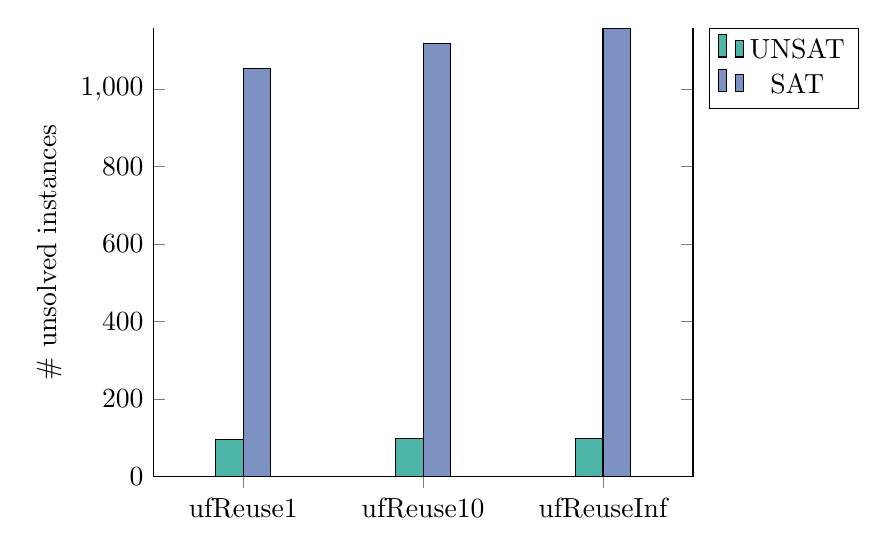
\begin{tikzpicture}
        \begin{axis}[
        legend pos=outer north east,
        enlargelimits={abs=0.5},
        ybar=0pt,
        ymin=0,
        axis x line*=bottom,
        xtick=data,
        xticklabels={ufReuse1, ufReuse10, ufReuseInf},
        xlabel={},
        ylabel={\# unsolved instances}]
        ]
        
        % UNSAT
        \addplot+[black, fill=KITgreen70]
        coordinates {
            (1,96)
            (2,97)
            (3,97)};
        
        % SAT:
        \addplot+[black, fill=KITblue70]
        coordinates {
            (1,1053)
            (2,1119)
            (3,1157)};
        
        \addlegendentry{UNSAT}
        \addlegendentry{SAT}
        \end{axis}
    \end{tikzpicture}
    \caption{Number of unsolved instances (both SAT and UNSAT) for fresh UF on every appearance (ufReuse1), fresh UF on every tenth appearance (ufReuse10) and the same UF for all appearances (ufReuseInf)}
    \label{fig:evaluation:ufreuse:solved_instances}
\end{figure}

\section{Unsatisfiable Instances}
The benchmark set considered contained a total of 15264 unsatisfiable instances. It is worth noting that 9404 of those instances are solved by Boolector without the use of a SAT solver at all leaving 5860 instances to be solved by the SAT solver. A first comparison of Boolector and Ablector is given in Figure \ref{fig:evaluation:unsat:scatter} and \ref{fig:evaluation:unsat:scatter-big}. While the plots show that for certain instances Ablector seems to be slower than Boolector, we can also see a number of instances for which Ablector finds a solution while Boolector times out. Figure \ref{fig:evaluation:unsat:scatter-big} only shows the instances which had a runtime of more than 1s for either solver, thereby removing all time differences irrelevant to us.\\
Although we can very well evaluate the differences in running time in the two figures, the plots lack essential information on the number of benchmarks solved by either solver.
A better analysis of the number of instances (un)solved by Boolector and Ablector can be found in table \ref{tab:evaluation:unsat:solvedUnsolved}:
Here we see that Ablector, using the abstractions presented above, is able to solve 43 instances more than Boolector. Note that in numbers (not looking at overlap etc.) this is about $30\%$ of the instances for which Boolector times out.

\begin{table}[ht]
    \begin{center}
    \begin{tabular}{cc|c|c|c}
        &&\multicolumn{2}{c|}{Boolector}&\\
        &&unsolved&solved&\\ \hline
        \multirow{2}{*}{Ablector}&unsolved& 80 & 16 & 96 \\ \cline{2-5}
        & solved & 59 & 15109 & 15168 \\ \hline
        & & 139 & 15125 & 15264 \\
    \end{tabular}
    \end{center}
    \caption{Number of unsatisfiable instances solved by Boolector and Ablector}
    \label{tab:evaluation:unsat:solvedUnsolved}
\end{table}

\begin{figure}[]
    \centering
        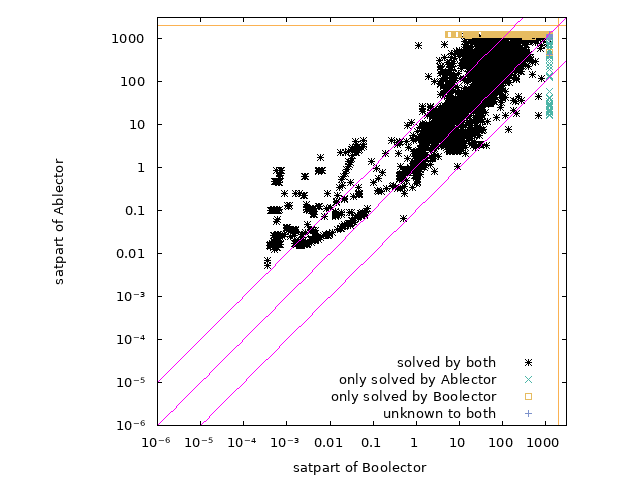
\includegraphics[width=0.7\textwidth]{plots/unsat/Boolector-vs-Ablector-satpart.png}
    \caption{\texttt{satpart} of Boolector vs \texttt{satpart} of Ablector in $\mu$s for unsatisfiable instances}
    \label{fig:evaluation:unsat:scatter}
\end{figure}

\begin{figure}[]
    \centering
        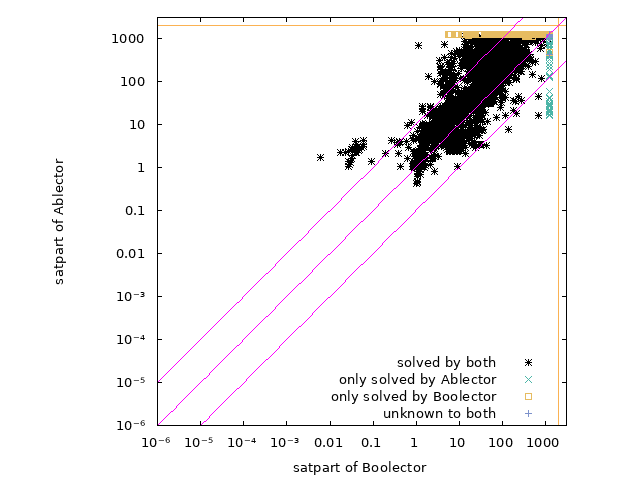
\includegraphics[width=0.7\textwidth]{plots/unsat/Boolector-vs-Ablector-satpart-big.png}
    \caption{\texttt{satpart} of Boolector vs \texttt{satpart} of Ablector in $\mu$s for unsatisfiable instances with satpart larger $1s$ in either dimension}
    \label{fig:evaluation:unsat:scatter-big}
\end{figure}
For any appearance of the \texttt{bvmul} and \texttt{bvsdiv} function within an instance we furthermore tracked the final abstraction level. Abstraction level 0 corresponds to the simple cases, level 1 corresponds to the msd based intervals, level 2 corresponds to the relations between functions and level 3 corresponds to the interval-wise full multiplication/division. If abstraction level 3 was reached, we further track the number of intervals added. This is of interest as it gives an estimate on the necessity of each refinement step: For example, if a refinement level would never appear as the final refinement step for an unsatisfiable instance, it is very unlikely that this abstraction is of much use. However looking at Figure \ref{fig:evaluation:unsat:level} we see that the final abstraction levels are somewhat distributed across the various abstraction steps and that all abstractions therefore help in solving certain instances.
Further, Figure \ref{fig:evaluation:unsat:interval} shows that for many instances full multiplication for a single interval (or very few intervals) are enough to produce the unsat result. This implies that the incremental, last refinement level also helps in solving certain instances.

\begin{figure}[ht]
    %\centering
    \begin{subfigure}[b]{0.5\textwidth}
        \centering
        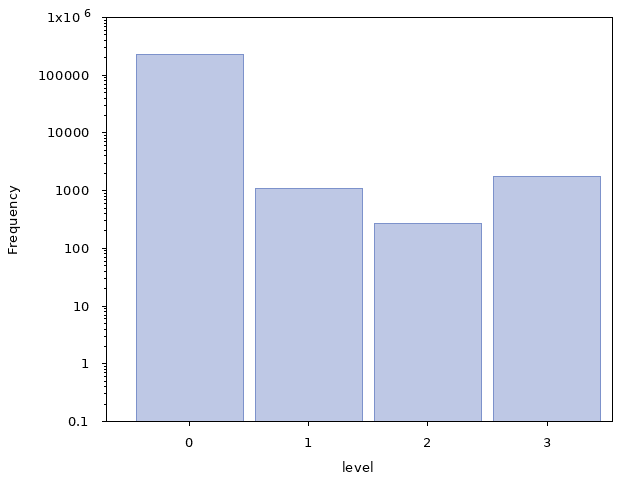
\includegraphics[width=\textwidth]{plots/unsat/level-MulNode.png}
        \caption{\texttt{bvmul}}
    \end{subfigure}
    \hfill
    \begin{subfigure}[b]{0.5\textwidth}
        \centering
        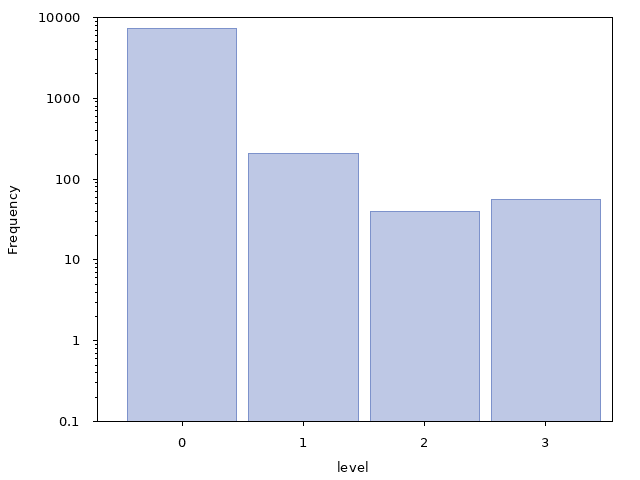
\includegraphics[width=\textwidth]{plots/unsat/level-SdivNode.png}
        \caption{\texttt{bvsdiv}}
    \end{subfigure}
    \caption{Final abstraction level of function applications: 0 are simple cases, 1 are bit shifts, 2 are UF relations and 3 is the interval-wise full multiplication/division step.}
    \label{fig:evaluation:unsat:level}
\end{figure}

\begin{figure}[ht]
    %\centering
    \begin{subfigure}[b]{0.5\textwidth}
        \centering
        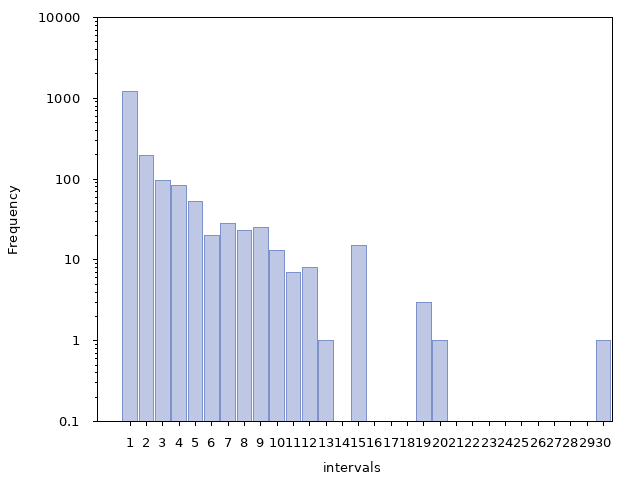
\includegraphics[width=\textwidth]{plots/unsat/bit-MulNode.png}
        \caption{\texttt{bvmul}}
    \end{subfigure}
    \hfill
    \begin{subfigure}[b]{0.5\textwidth}
        \centering
        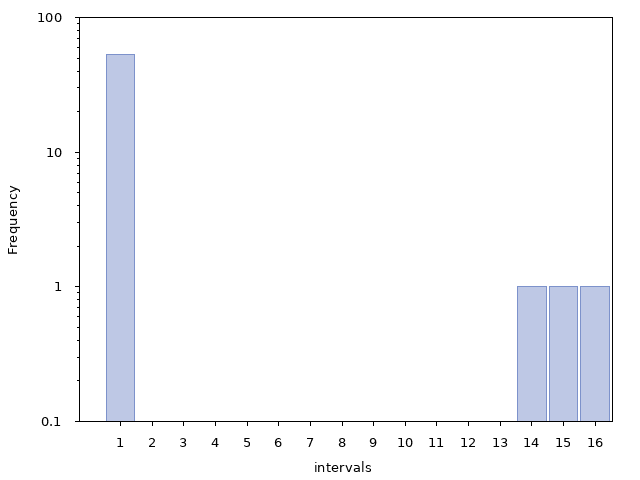
\includegraphics[width=\textwidth]{plots/unsat/bit-SdivNode.png}
        \caption{\texttt{bvsdiv}}
    \end{subfigure}
    \caption{Number of intervals added for multiplication/division in the final abstraction step.}
    \label{fig:evaluation:unsat:interval}
\end{figure}

%NOTE(steuber): Refinement time vs sat time?

\section{Satisfiable Instances}
For satisfiable instances on the other hand, Abletor's performance is worse than Boolector's: As we can see in Figure \ref{fig:evaluation:sat:scatter} and Table \ref{tab:evaluation:sat:solvedUnsolved}, Boolector is able to solve a lot of instances Ablector cannot currently solve and the running time Ablector takes for the solved instances cannot make up for this flaw.
It is also worth noting that, while about 500 timed out instances got stuck in the first refinement round, the rest of the timed out instances are evenly distributed across all refinement rounds.
\paragraph{}
While bounding the running time of each refinement round by an upper limit could avoid the problem of instances getting stuck in a certain step, we expect that the abstraction scheme's performance could further be improved in future work by integrating the abstractions directly into a solver like Boolector instead of building them as a layer on top. This would allow to make better use of the under-approximation techniques that are completely ignored for most abstraction steps in the current abstraction scheme.

\begin{figure}[]
    \centering
        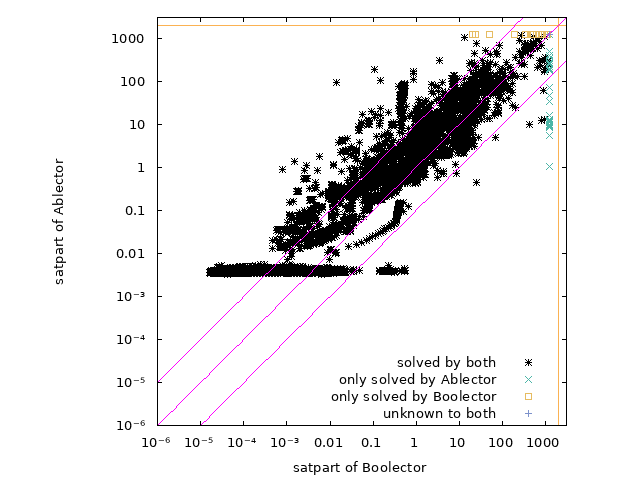
\includegraphics[width=0.7\textwidth]{plots/sat/Boolector-vs-Ablector-satpart.png}
    \caption{\texttt{satpart} of Boolector vs \texttt{satpart} of Ablector in $\mu$s for satisfiable instances}
    \label{fig:evaluation:sat:scatter}
\end{figure}

\begin{table}[ht]
    \begin{center}
    \begin{tabular}{cc|c|c|c}
        &&\multicolumn{2}{c|}{Boolector}&\\
        &&unsolved&solved&\\ \hline
        \multirow{2}{*}{Ablector}&unsolved& 579 & 474 & 1053 \\ \cline{2-5}
        & solved & 73 & 3400 & 3473 \\ \hline
        & & 652 & 3874 & 4526 \\
    \end{tabular}
    \end{center}
    \caption{Number of satisfiable instances solved by Boolector and Ablector}
    \label{tab:evaluation:sat:solvedUnsolved}
\end{table}
\chapter{Conclusion}
\label{ch:Conclusion}
In this work, we introduced a novel approach to solving quantifier free bitvector problems in SMT-LIB's \texttt{QF\_BV} theory. The approach is based on abstraction methodologies previously used for various other problems in logic and specifically in SMT.
On the one hand, we presented numerous abstractions for 3 comparatively costly funcitons of the bitvector theory, on the other hand, we proposed a simple theoretical framework allowing a proof of correctness for the presented abstractions.
While we saw that the presented approach performs better than Boolector in deciding unsatisfiable bitvector problems, solving 43 instances more, the implemented prototype is not yet competitive for satisfiable instances. This is of course in some way a natural result, as over-approximations usually improve the solver runtime on unsatisfiable (and not on satisfiable) instances.

\paragraph{Future Work}
With the abstraction's correctness proved and the abstraction's performance evaluated through the current prototype, one could now implement the abstraction scheme directly into a SMT solver like Boolector making use of interleaved under- and over-approximations. We expect that this might enhance the solver's performance sufficiently to be competitive for both satisfiable and unsatisfiable instances.
Additionally, a time limit for each refinement round could be introduced in order to avoid cases where the solver gets stuck in some specific refinement step. For this, a detailed parameter analysis will be necessary to find a time limit that keeps the abstraction steps effective while avoiding dead ends. Finally, it is left to investigate whether a \textit{don't care reasoning} strategy similar to the one used for Lemmas on Demand in Boolector \cite{NiemetzPreinerBiere-FMCAD14} could improve the abstraction refinement procedure's performance.

%% --------------------
%% |   Bibliography   |
%% --------------------

%% No cite entries
\nocite{fondements-logique}

%% Add entry to the table of contents for the bibliography
\printbibliography[heading=bibintoc]

%% ----------------
%% |   Appendix   |
%% ----------------
\appendix
\begin{appendices}
\chapter{Appendix}
\label{chap:appendix}

\section{Reproducibility}
\label{sec:appendix:reproducibility}
\paragraph{Software}
For alle experiments a modified version of \texttt{Boolector 3.0.1-pre} was used.
More specifically we modified commit \texttt{f689fbbfe820392d35e26be368f9d87d2dbdb037} so that we could measure the time of the \texttt{check-sat} instruction.
As underlying SAT-solver Lingeling with version \texttt{bcj 78ebb8672540bde0a335aea946bbf32515157d5a} was used.
All software packages were compiled using the included cmake scripts which have the highest optimization levels enabled.\\
For the final experiments presented in chapter \ref{ch:evaluation} Ablector was used in the version available in commit 79584caeb4b7ea27ac3e80153b167c36d434232e available at \url{https://github.com/samysweb/ablector}.

\paragraph{Machine}
All experiments were executed on a cluster of 20 identical compute nodes each containing 2 Intel Xeon E5430 @ 2.66GHz CPUs.
Each compute node had a total of 32GB of RAM.
The SMT benchmark files were stored on a RAID system connected to the cluster.

\paragraph{Benchmark execution}
2 jobs were run in parallel on each compute node with the timeout set to 1200 seconds
this posed no caching issues as they were run on seperate CPU sockets
\footnote{Early on we ran up to 8 experiments on a single node to make use of the available cores however this seemed to produce caching issues slowing down the experiment times}.
For time surveillance and measurements we used the runlim utility \cite{runlim}.
All benchmarking scripts and the log results can be obtained at \todo{Insert experiment repo once uploaded}.
\todo{Publish repos!}
\end{appendices}

\end{document}
